\chapter{Virtuális gépen kialakított tesztrendszerek}
A felhőberendszerbe való integrálás előtt két tesztet végzek Ubuntu VM-eken, amik a működés szempontjából fontosak lesznek.
\section{Azonos konténerrel egy drónvezérlés}
Az első ilyen teszt egy a TMIT tanszék egyik előre készített konténerével lesz, ez a DockerHub-on megtalálható \emph{bmehsnlab/aruco\_detect\_image\_v2} konténer. Ebbe a konténerbe bele van építve a videó stream, a kép feldolgozása, ami aruco kódokat detektál, a Mavros node működése és az irányító program.
Ezen konténerek indítása előtt ki kell adnunk az \emph{xhost} parancsot, mivel az X szerveren keresztül kommunikálnak egymással. Az X szerver kommunikációjához a konténereknek felcsatoljuk a \emph{/tmp/.X11-unix} fájlt.
\begin{lstlisting}[caption={Azonos konténerek indítása négy különböző feladattal és az X szerveren való kommunikációt megvalósítva}]
xhost +
docker run --net=host -v /tmp/.X11-unix:/tmp/.X11-unix --name stream bmehsnlab/aruco_detect_image_v2
docker run --net=host -v /tmp/.X11-unix:/tmp/.X11-unix --name dtctor bmehsnlab/aruco_detect_image_v2
docker run --net=host -v /tmp/.X11-unix:/tmp/.X11-unix --name mavros bmehsnlab/aruco_detect_image_v2
docker run --net=host -v /tmp/.X11-unix:/tmp/.X11-unix --name cntrol bmehsnlab/aruco_detect_image_v2
\end{lstlisting}
\begin{figure}
	\centering
	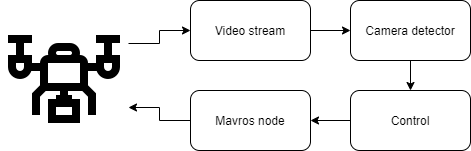
\includegraphics[width=\linewidth]{figures/local.png}
	\caption{Négy azonos konténerrel drónirányítás}
	\label{fig:azonos}
\end{figure}
A teszt architektúrája a \ref{fig:azonos}. képen látható. A teszt sikeresnek mondható, mivel a drónt sikerült irányításra bírni, illetve az optikai adatfolyamot fel tudta dolgozni az aruco kódfeldolgozó, habár aruco kódok nem voltak a szimulált világban.

\section{Két VM-en több drón szimulációja és vezérlése}
A következő teszten egy host OS-ből indított két VM-en teszteltem a több drón irányítását manuálisan. A teszthez telepítettem a VM-eken a fejezetben már felsorolt szoftvereket és környezeteket és a \ref{lst:multi}. listázásban bemutatott módon több drónt szimulációt is indítottam egy VM-en. Majd ezeket a földi irányítóállomás szimulátorával manuálisan vezéreltem. A teszt architektúrája a \ref{fig:ketvm}. ábrán látható.
\begin{figure}
	\centering
	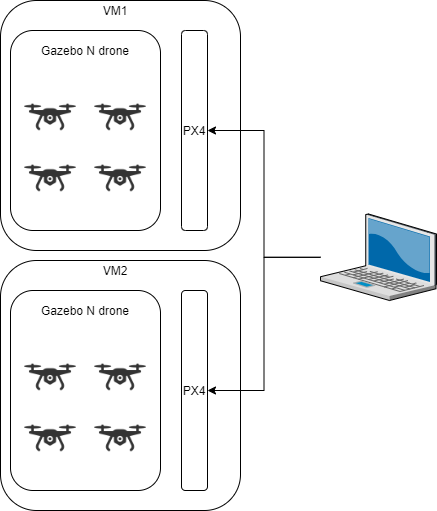
\includegraphics[height=10cm]{figures/multi-control.png}
	\caption{Két VM-en több drón irányítása}
	\label{fig:ketvm}
\end{figure}
